\documentclass{article}
\usepackage{graphicx}
\usepackage{Sweave}
\usepackage{amssymb,amsfonts,amsmath}
\usepackage[natbib=true, bibstyle=authoryear, citestyle=authoryear-comp]{biblatex}
\usepackage[T1]{fontenc}
\usepackage[utf8]{inputenc}
\usepackage{aeguill}
\usepackage{inputenc}
%\usepackage{hyperref}


\setkeys{Gin}{width=\textwidth}

\newcommand\R{\rule{0pt}{2.5ex}}
\newcommand\B{\rule{0pt}{-1ex}}
\renewcommand{\belowcaptionskip}{1ex}

\setlength{\parindent}{0cm}

\bibliography{/home/olive/Boulot/biblio/db/biblio}

%%%%%%%%%%%%%%%%%%%%%%%%%%%%%%%%%%%%%%%%%%%%%%%%
\title{Elevational distribution patterns differ between exotic and native birds in Reunion Island}
%\author{Olivier Flores}

%%%%%%%%%%%%%%%%%%%%%%%%%%%%%%%%%%%%%%%%%%%%%%%%

\begin{document}
%<<echo=false,label=data,cache=true,include=false>>=
%chunk="data"
%source("../R/data_zoizo.r")
%@ 

\maketitle

\noindent

\begin{abstract}
%Although biological invasions are one of the most important changes in ecological dynamic, they have been rarely investigated along elevational gradients. The objective of this study was to compare the distributions of exotic versus native birds on a same broad elevational gradient. Field studies were conducted on the leeward side of Reunion Island (Mascarene Archipelago, Western Indian Ocean) between 20 and 2880 m at 363 sampling points. Species richness and abundances of bird species were surveyed during the nesting season using 20 min count at each point. Mean elevational position and elevational amplitude were measured for each species and a Mean Distribution Index was computed as the number of bird species having their mean elevation within each 100 m elevational band. The data show that (1) the elevational variation of native species richness is hump-shaped, whereas the richness of exotic bird species does not vary in the first half of the gradient; (2) the elevational amplitude and maximum elevation do not differ significantly between exotic and native birds, but the mean and minimum elevations are higher for native birds; and (3) the most suitable vegetation types are found in the ‘rural landscapes’ belt for the exotic bird communities, and in the higher belt of ‘forest and pastures’ for the native ones. Even if history can appear too short to permit niche expansion of the more recent introduced species, we can underline the exotic species preference for anthropogenic landscapes and their large amplitude in elevation. 
\end{abstract}


%%%%%%%%%%%%%%%%%%%%%%%%%%%%%%%%%%%%%%%%%%%%
\section*{Introduction}

The conspicuous ecological changes that occur along elevational gradients have drawn the attention of an increasing number of researchers. Most hypotheses which attempted to explain biological responses to elevational gradients were formally based on a single bio-physical factor such as productivity, habitat diversity, environmental stress, resource availability or competition (e.g. Rahbek, 1995; Heaney, 2001). Others underlined the role of anthropogenic pressure or ecological and evolutionary processes (e.g. Myers \& Giller, 1988). 
Surprisingly, studies on species distribution along elevational gradients scarcely pay attention to the status of the involved species, i.e. either exotic or native (but see Tassin \& Rivière, 2003; Tassin et al., 2004), despite of the increased importance of the impact of introduced species on biodiversity (Vitousek et al., 1997). The same can be said of studies on latitudinal gradients (but see Sax, 2001). Considering the theoretical framework of biological invasions, investigations on the distribution of exotic species along broad ecological gradients should enable us to predict invasion patterns. 
Birds, widely introduced throughout the world and having colonized most vegetation types (Long, 1981), are a relevant taxon for studying the comparative distribution of exotic versus native species along elevational gradients. Exotics may be defined as species that have been introduced by humans, or have been able to expand their range because of anthropogenic disturbances, into geographical regions in which they were not historically present (Sax, 2001). Birds have been widely used as models in studies on the variation of species richness with elevation (Thiollay, 1980; Patterson et al., 1998; Benning et al., 2002 ; Prodon et al., 2002). The elevational range of bird communities is also of special interest as it is one of the dimensions of the niche of a species, and it is linked to flexibility in habitat or food choices, ability to coexist with different species, and physiological tolerance (Prodon et al., 2002). Last, the mean elevational position can be considered to be an indicator for determining one of the optimal vegetation types of a species. 
In this paper, we compare elevational patterns of bird species along an elevational gradient sufficiently broad to reveal possible different responses between exotic and native birds. We chose to analyse a slope of Reunion Island that presents one of the widest bio-climatic gradients within any oceanic island, i.e. 0 to more than 3000 m on a distance of only 20 km. In addition, studies in this kind of oceanic islands may contribute to understanding the potentially huge impact of biological invasions (Loope \& Mueller-Dombois, 1989). This paper focuses on a specific question: do elevational distribution patterns vary between exotic and native bird communities? Consequently, for each one of these groups, we compared species richness pattern; maximal elevation, minimal elevation, elevational amplitude, and the variation of mean elevational positions with elevational bands. We used the word elevation instead of altitude, though both elevation and altitude are used as synonyms, as elevation is meters above sea level and is more correct than altitude which is meters above ground.



%Nineteen native bird species on the island among which five are classified as endangered (Coracina newtoni, Pseudobulweria aterrima, Circus
%maillardi, Pterodroma baraui, Psittacula echo. Twenty exotic species have established populations on the island. 

%%%%%%%%%%%%%%%%%%%%%%%%%%%%%%%%%%%
\section*{Material and methods}

\subsection*{Studied area}
Reunion Island is part of the Mascarene volcanic archipelago, situated in the Western Indian Ocean (55°30’ E and 21°05’ S)(Fig. 1). This oceanic island appeared three million years ago. In the centre of the island, a plateau (Plaine des Caffres, $\approx$2000 m) is flanked by two volcanoes (Piton de la Fournaise, 2631 m; Piton des Neiges, 3069 m), the sides of which slope steeply towards the sea. There is a very steep climatic gradient: the average minimum ground temperature falls below 0°C above 1500 m in August, above 1800 m from June to October, and above 2300 m all year round; at the highest point, the temperature ranges from -10°C to +26°C \citep{Cadet1974,Raunet1991}.
The studied area, located on the leeward side of the island had a slope of about 0.15 m per m and an annual rainfall ranging from 500 mm at sea level to 2000 mm on the highest mountain slopes \cite{Raunet1991}. The land is roughly organized through a land use gradient into a succession of elevational belts \citep{Cadet1980} urbanised areas (0-50 m a.s.l.), herbaceous savannah (50-300 m), sugarcane monoculture (300-800 m), rural landscapes with diversified crops (800-1200 m), primary forest mixed with pastures and planted forests (1200-1800 m), heathlands dominated by ericaceous plants (1800-2600 m), and bare soils with a very sparse vegetation of herbaceous species (2600-3069 m) (Fig. ??). Above 1200 m, about 60 % of the original primary forest and 80 % of the original heathlands have been preserved from clearing (Strasberg et al., 2006).

\subsection*{Sampling}
The transect was sampled through one survey during the breeding season (December, 1997 - April, 1998), using 363 sample points spread along an elevational gradient from 20 m to 2880 m (Fig. ??). Further prospecting between 2880 and 3069 m (Piton des Neiges) revealed no bird presence. This was due to of a lack of vegetation, except for scarce amounts of native herbs and weeds. Sampling points were equally distributed all along the elevational gradient, with a mean elevational distance of 8 m between two successive elevations, and a distance of at least 250 m between two successive count points, a mean sampling pressure of 12.7 count points per 100 m elevational band, and covering the overall diversity of vegetation types. Under-sampling of some elevational bands or vegetation types would have brought about an under-evaluation of species richness along the considered ecological gradient \citep{Prodon1981,Rahbek1997,Patterson1998}. Depressions, ridges and mires were avoided in order to avoid extremely wet or dry places. We also avoided places too close to feeding troughs in grasslands as they attract granivorous bird species. We assume that most of the birds were sampled near their nesting sites. In order to limit sampling bias, the different ecosystems found at each 100~m elevational band were surveyed so as not to miss individual bird species specific to individual ecosystems. 

%An equal sampling effort may still result in sampling unequal proportions of the total richness, which may in turn affect the elevational species richness pattern once interpolation is used \citep{Colwell1994}. One reason for this is that, in this case, richness towards the boundaries only consists of observed species, whereas at other elevations richness consists of observed species plus the species added by interpolation (Grytnes \& Vetaas, 2002)

Data were collected using the point count method during the nesting period \citep{Blondel1970}. Data were collected between 5.30 a.m. and 10.30 a.m. Elevation was recorded using an electronic altimeter of a $\pm$ 10 m accuracy. Every terrestrial bird species observed within a radius of 150 m around each count point was recorded on a paper form. The duration of each count was 20 minutes. The nomenclature and biogeographical status of the birds was described in accordance with \citep{Sinclair1998}.

%\subsection*{Analysis}
%Elevation patterns of species composition of exotic versus native bird communities were based on elevational bands of 100 m investigated in three different ways: (1) the variation of species richness with elevation was analyzed, (2) the distribution of species along the elevational gradient was characterized with regards to mean elevation and range, and (3) the current optimal elevational band of each species in terms of reproductive success and fitness. Most studies on elevational gradients focus on the variation of species richness with elevation but do not give any information on the mean elevational position, that is to say the optimal elevational position of the studied taxa (Rahbek, 1997; Paterson et al., 1998; Odland \& Birks, 1999; Kessler, 2000; Grytnes, 2003). In terms of conservation, it appears sound to identify those elevational bands that are optimal for a great number of species, even if we must consider that some species have been displaced from their optimal location by human land use and conversely that human land use has added resources to the landscape. The investigation of the elevational distribution of the mean elevations of studied species yields information that the mere examination of variation of species richness with elevation will not provide. Therefore, for each 100m elevational band, we computed a Mean Distribution Index MDI which is the number of bird species having their mean elevation in band. Only species recorded in more than five point counts were used in the computation.
%Comparisons between exotic and native species were performed using the Man-Whitney test. Correlations were computed using Pearson product-moment correlation coefficients and tested using the Bonferroni adjusted probability. All statistical analyses were computed using R software.


We calculated the weighted mid-point of species distribution as the average of elevation where a species was recorded weighted by the number of times it was detected. 


We compared observed species richness in the two groups of bird species (native and exotic) to two different null models based on random permutations of the original dataset  \cite{Gotelli2000}. In both models, species overall abundance, that is the total number of records, was preserved in each permutation, in order to account for observed differences in species commonness and detectability. The main difference between the two null models was in the treatment of site carrying capacity which is defined here as the number of species observed locally. In the first nul model, sites were considered as equally suitable for bird diversity. In this  case, the randomization suppresses any structure that could exist in the data due to relationships between species and their environment in a broad sense. The random pattern obtained mimics the distribution of species richness not accounting for these relationships. In the second null model, site totals, that is local species richness, were preserved by the randomization procedure. This model holds account for differences in sites to support bird species diversity, in relation with habitat carrying capacity and suitability. The obtained random pattern thus takes into account both species commonness and site suitability. The number of species present locally is preserved, but bird diversity is randomly assembled according to species status. It thus allows us to explore the differences in elevational patterns between of species richness between native and exotic birds under the constraint of observed overall species richness. For each model, we performed a large number of permutations ($n=1999$) in order to obtain confidence intervals on simulated species richness. 



%%%%%%%%%%%%%%%%%%%%%%%%%%%%%%%%%%%
\section*{Results}

We detected 22 bird species over the 363 sampling points, with a mean of 4.3 species per point and 10.4 species per elevational band along the gradient.  Fourteen species were exotic and eight native (Table \ref{species}). The number of records varied widely across species between 1 for two species (\textit{Coturnix chinensis, Phedina borbonica}) and 268 for \textit{Zosterops borbonicus} (mean: 71.2 $\pm$ s.d.: 77.8, Fig. \ref{boxalti}). 

Amplitude in elevational ranges was high. Elevational amplitude exceeded 2000~m for five species and 1000~m for 15 species (Table 1). The largest elevational amplitude observed within native species was registered for \textit{Zosterops borbonicus} (92 \% of the gradient) and within exotic species for \textit{Acridotheres tristis} (83 \%). The lowest elevational amplitude observed within native species was registered for \textit{Circus maillardi} (20 \%) and for \textit{Perdicula asiatica} within exotic species (8 \%). The distribution of weighted mid-points for bird species along the gradient was highly concentrated between 1000 and 1500 m, with the exception of three exotic species (Fig. \ref{boxrange}). However, the weighted mid-point and minimum elevation were higher within native species ($p=0.034$ and $p=0.024$). By contrast, elevational amplitude and maximum elevation did not differ significantly between native and exotic species ($p=0.534$ and $p=0.254$ respectively, Fig. \ref{boxrange}). No difference in the variability of species distribution was observed across the two groups: Bartlett test's of variance homogeneity showed that the variability was similar in the two groups for the four tested variables.

The variation of species richness with elevation differed significantly between exotic and native species (Fig. \ref{Sgam}). 
The total species richness observed within 100-m elevation bands varied between 2 and 19 (10.4$\pm$5.5, Fig. \ref{Sgam}.a). Total richness showed a unimodal mid-elevational peak between 1000 and 1200~m. When species were considered separately according to their status,  species richness varied between 0 and 7 for native birds (3.5$\pm$2.2), and between 1 and 12 (6.9$\pm$3.9) for exotic birds (Fig. \ref{Sgam}.b). Species richness showed different elevational patterns across the two groups. Species richness of native birds showed a unimodal mid-elevational peak around 1200~m, whereas richness for exotic birds species showed a low-elevation plateau with a small mid-peak also around 1200~m. Exotic species were more numerous than native birds up to mid-elevation, whereas species richness was similar in the groups at higher altitudes (Fig. \ref{Sgam}.b). According to richness patterns, three zones could be defined: (1) from 0 to 1000 m, there was a significant difference between exotic and native species, both in the number of species contacted and in their variation pattern, as native species increased with the elevational gradient from two to seven while the exotic ones remained at a high level (around 9 species ); (2) from 1000 to 1500 m, richness of both exotic and native species presented a peak (around 9 and 6 species, respectively); (3) from 1500 to 3000~m, richness in exotic and native species decreased to 1-3 species. 


In order to explore species co-occurence according to their status, we compared species richness to random patterns obtained by simulation. Null patterns showed more uniform variations with respect to elevation when sites were considered equally suitable (Fig. \ref{Snull}.a\&b) than when differences were maintained. In the latest case, hump-backed variations were obtained for both native and exotic birds with a peak of expected diversity around 1500~m in both groups (Fig. \ref{Snull}.c\&d). This finding was particularly true at high elevations when observed species richness was low (Fig. \ref{Sgam}.a) in relation with harsh environmental conditions.

Values occurring within the simulated 95\% confidence band for the random pattern indicated elevation bands where species richness was not statistically different from random patterns of species assemblage (Fig. \ref{Snull}). Native species richness was significantly lower than random expectations at low altitude for both null hypotheses (Fig. \ref{Snull}.a\&c), over 1700~m for the equal sites hypothesis (Fig. \ref{Snull}.a), and mostly between 1700 and 2200 m for the unequal sites hypothesis (Fig. \ref{Snull}.c). Regarding exotic birds, few cases excepted, observed species richness was lower than expected under randomness under the two null hypotheses (Fig. \ref{Snull}.b\&d).


Diversity in native birds was lower than expected under the null model at low elevation. 



%%%%%%%%%%%%%%%%%%%%%%%%%%%%%%%%%%%
\section*{Discussion}

%\printbibliography
\section*{Tables}

% latex.default(era, cdec = c(0, rep(0, 5)), caption = "Summary of species elevation patterns",      ctable = FALSE, label = "era", file = "tables/zoizos_era.tex") 
%
\begin{table}[!h]
\caption{Summary of species elevation patterns. Occurrence: number of times the species was recorded. Mean : average elevation where the species was observed. Weighted mean: average altitude weighted by the number of times the species was recorded at each site. Min., Max.; minimum and maximum elevation at which the species was observed.\label{era}} 
\begin{center}
\begin{tabular}{lccccc}
\hline
\multicolumn{1}{l}{\R Species}&\multicolumn{1}{c}{Occurrence}&\multicolumn{1}{c}{Mean (m)}&\multicolumn{1}{c}{Weighted mean (m)}&\multicolumn{1}{c}{Min.}&\multicolumn{1}{c}{Max.}\tabularnewline
\hline
\R ACTR&$168$&$1084$&$1123$&$  20$&$2400$\tabularnewline
CIMA&$  6$&$1058$&$1049$&$ 800$&$1370$\tabularnewline
COCH&$  1$&$1010$&$1010$&$1010$&$1010$\tabularnewline
COCO&$ 33$&$1267$&$1307$&$ 320$&$1700$\tabularnewline
COFR&$ 57$&$1115$&$ 974$&$ 185$&$1660$\tabularnewline
ESAS&$ 88$&$1001$&$ 987$&$  60$&$1720$\tabularnewline
FOMA&$268$&$1051$&$1033$&$  20$&$2250$\tabularnewline
FRPO&$  2$&$ 128$&$ 142$&$  70$&$ 185$\tabularnewline
GEST&$109$&$ 840$&$ 804$&$  20$&$1620$\tabularnewline
HYBO&$ 67$&$1405$&$1410$&$ 620$&$2560$\tabularnewline
MAMA&$  5$&$1528$&$1615$&$1240$&$1705$\tabularnewline
PADO&$ 72$&$1128$&$1202$&$  65$&$1960$\tabularnewline
PEAS&$ 16$&$ 117$&$ 119$&$  50$&$ 290$\tabularnewline
PHBO&$  1$&$1495$&$1495$&$1495$&$1495$\tabularnewline
PLCU&$ 32$&$ 580$&$ 606$&$  65$&$1345$\tabularnewline
PYJO&$ 72$&$ 794$&$ 805$&$  65$&$1690$\tabularnewline
SATE&$202$&$1590$&$1601$&$ 270$&$2880$\tabularnewline
STPI&$ 34$&$1181$&$1225$&$ 100$&$2150$\tabularnewline
TEBO&$ 18$&$1307$&$1336$&$ 900$&$1680$\tabularnewline
TUNI&$ 41$&$ 832$&$ 808$&$  35$&$1700$\tabularnewline
ZOBO&$229$&$1371$&$1347$&$  60$&$2700$\tabularnewline
ZOOL&$ 45$&$1391$&$1388$&$ 620$&$2600$\tabularnewline
\hline
\end{tabular}
\end{center}
\end{table}



%%%%%%%%%%%%%%%%%%%%%%%%%%%%%%%%%%%
\section*{Figure legends}

Figure \ref{boxalti}: Box-and-whisker plots indicating the median, first and third quartiles and values outside inter-quartile range of elevations where species were detected. Species are sorted by order of median evelation. Blue indicates native species, , and red exindicate exotic species. Species are labelled with the first two letters of the genus and species names (see Table \ref{species}).

Figure \ref{boxrange}: Four features of species distributions with respect to elevation in native and exotic species : (a) weigthed mid elevation point (average elevation where the species was detected weighted by number occurences), (b) elevation amplitude (difference between highest and lowest elevation of detection), (c) minimum elevation where the species was detected and (d) maximal elevation of detection. Box-and-whisker plots indicate the median, first and third quartiles and values outside inter-quartile range. Symbols indicate individual values ($n=22$ species), open symbols indicate species with less than 5 records in dataset ($n=3$ species, see Table \ref{era}).

Figure \ref{Sgam}: Elevation patterns of species richness : (a) total and (b) according to species status, native or exotic. Richness is calculated here per 100-m elevation band as the number of species detected within the band. Dotted lines indicate generalized additive models fits (GAM) with colored bands showing the 95\% confidence interval on estimated richness. 

Figure \ref{Snull}: Comparison between observed richness (dots) within 100-m elevation bands for native (a. \& c.) and exotic (b. \& d.) birds and expected species richness under two different null models (95\%-confidence band): (a. \& b.) nul model with equally suitable sites hypothesis, individual observations were randomized while preserving species overall abundance in the dataset (column margin), (c. \& d.) nul model with unequal sites carrying capacity hypothesis where individual observations were randomized while preserving both overall species abundance in the dataset and local species richness (row margin).

%%%%%%%%%%%%%%%%%%%%%%%%%%%%%%%%%%%
\section*{Figures}

\begin{figure}
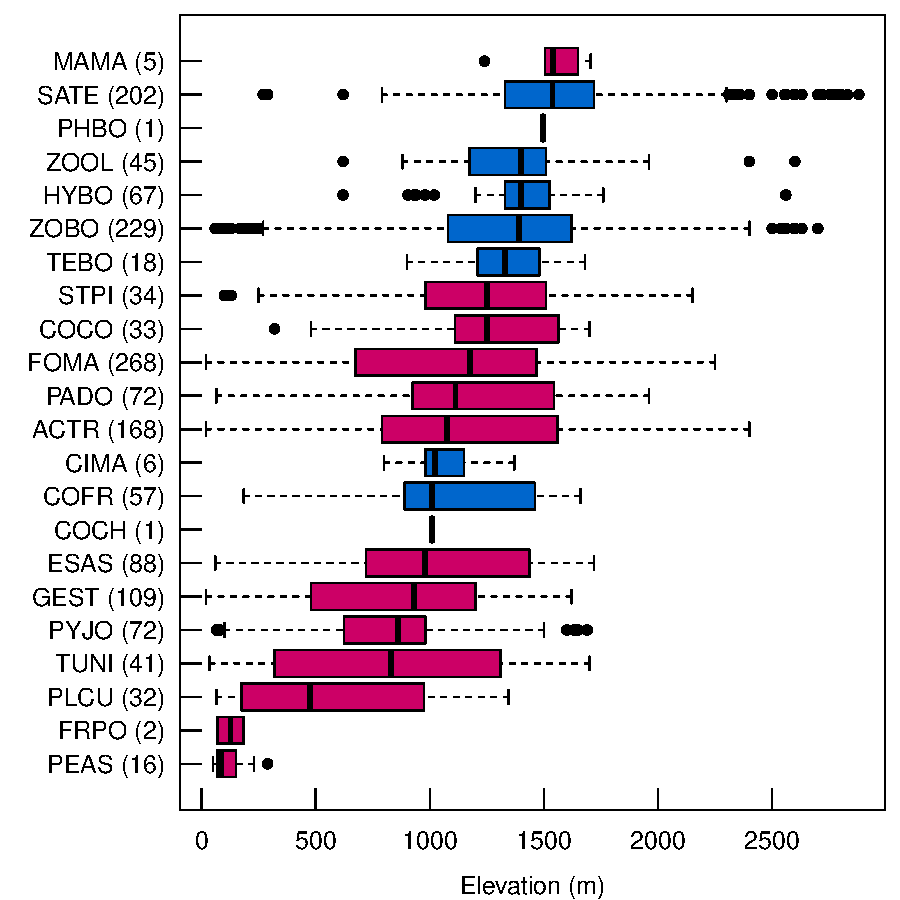
\includegraphics{figures/zoizos-boxalti}
\caption{\label{boxalti}}
\end{figure}

% % % % % % % % % % % % % % % % % % % % % % % % % %
	
\begin{figure}
\hspace{-2cm}
\begin{tabular}{cc}
(a) & (b) \\
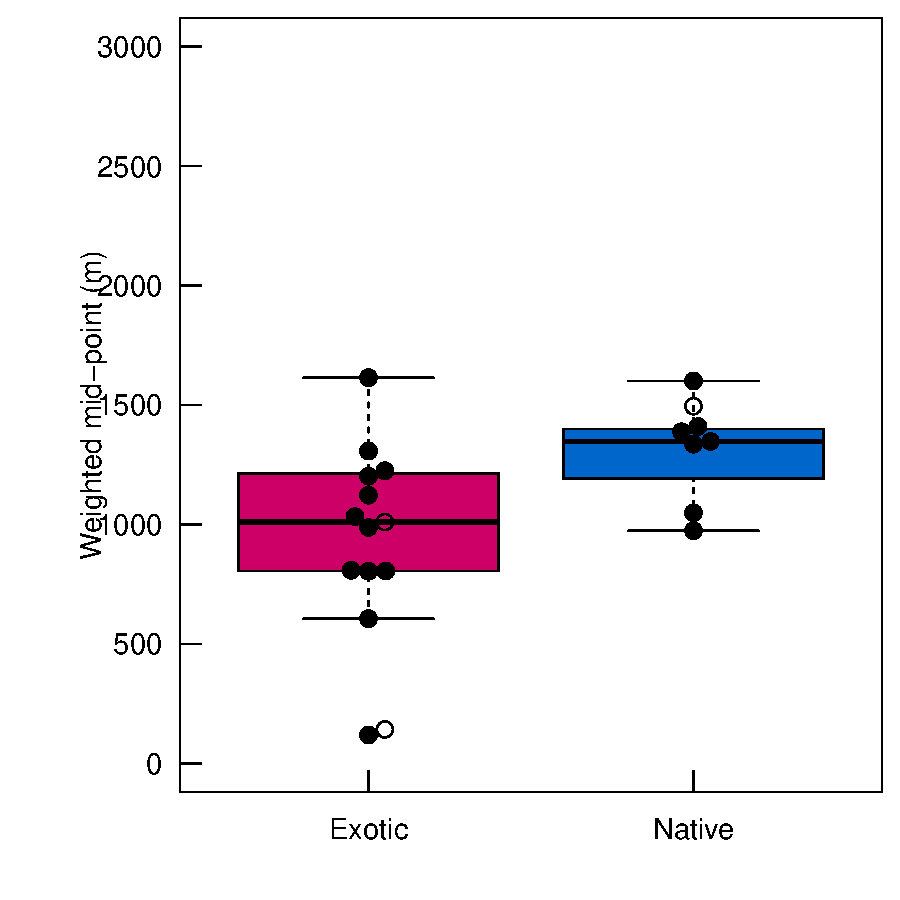
\includegraphics[width=0.7\textwidth]{figures/zoizos-boxwmalt}&
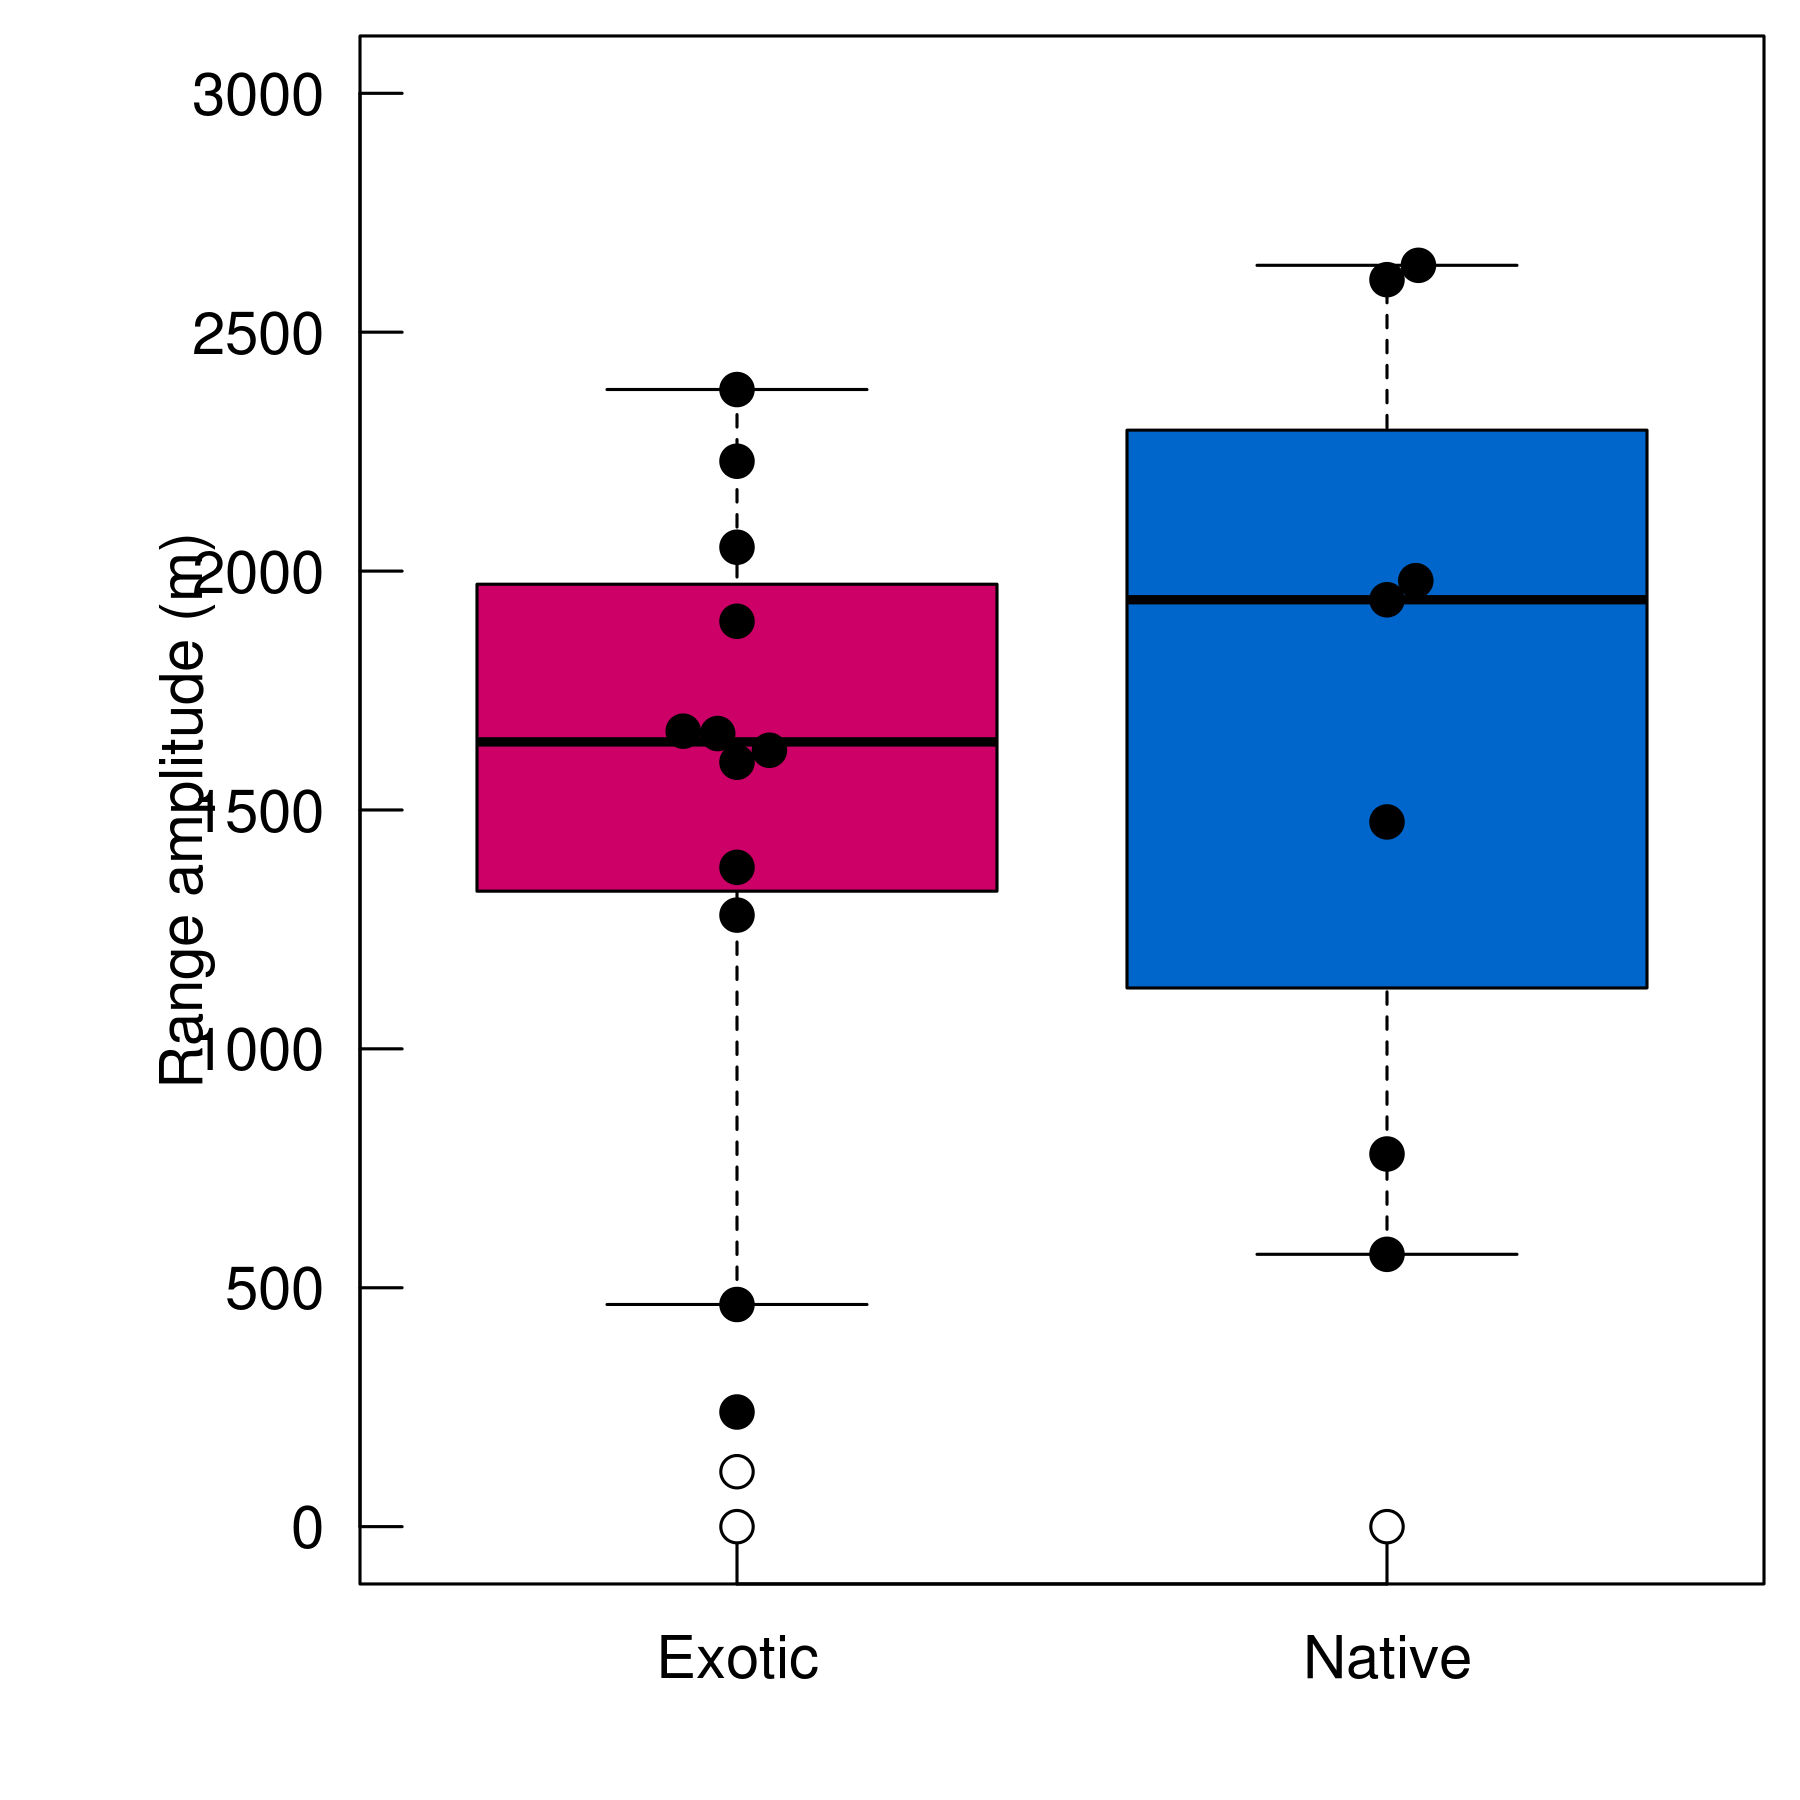
\includegraphics[width=0.7\textwidth]{figures/zoizos-boxampl}\\
(c) & (d) \\
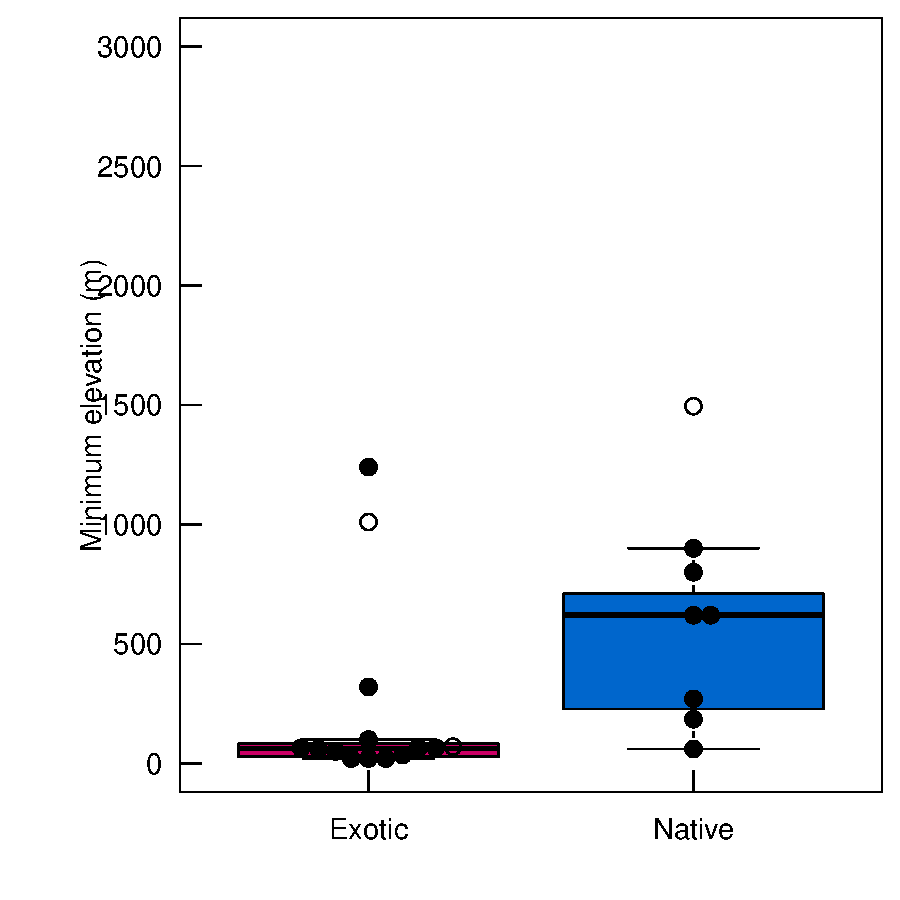
\includegraphics[width=0.7\textwidth]{figures/zoizos-boxmin}&
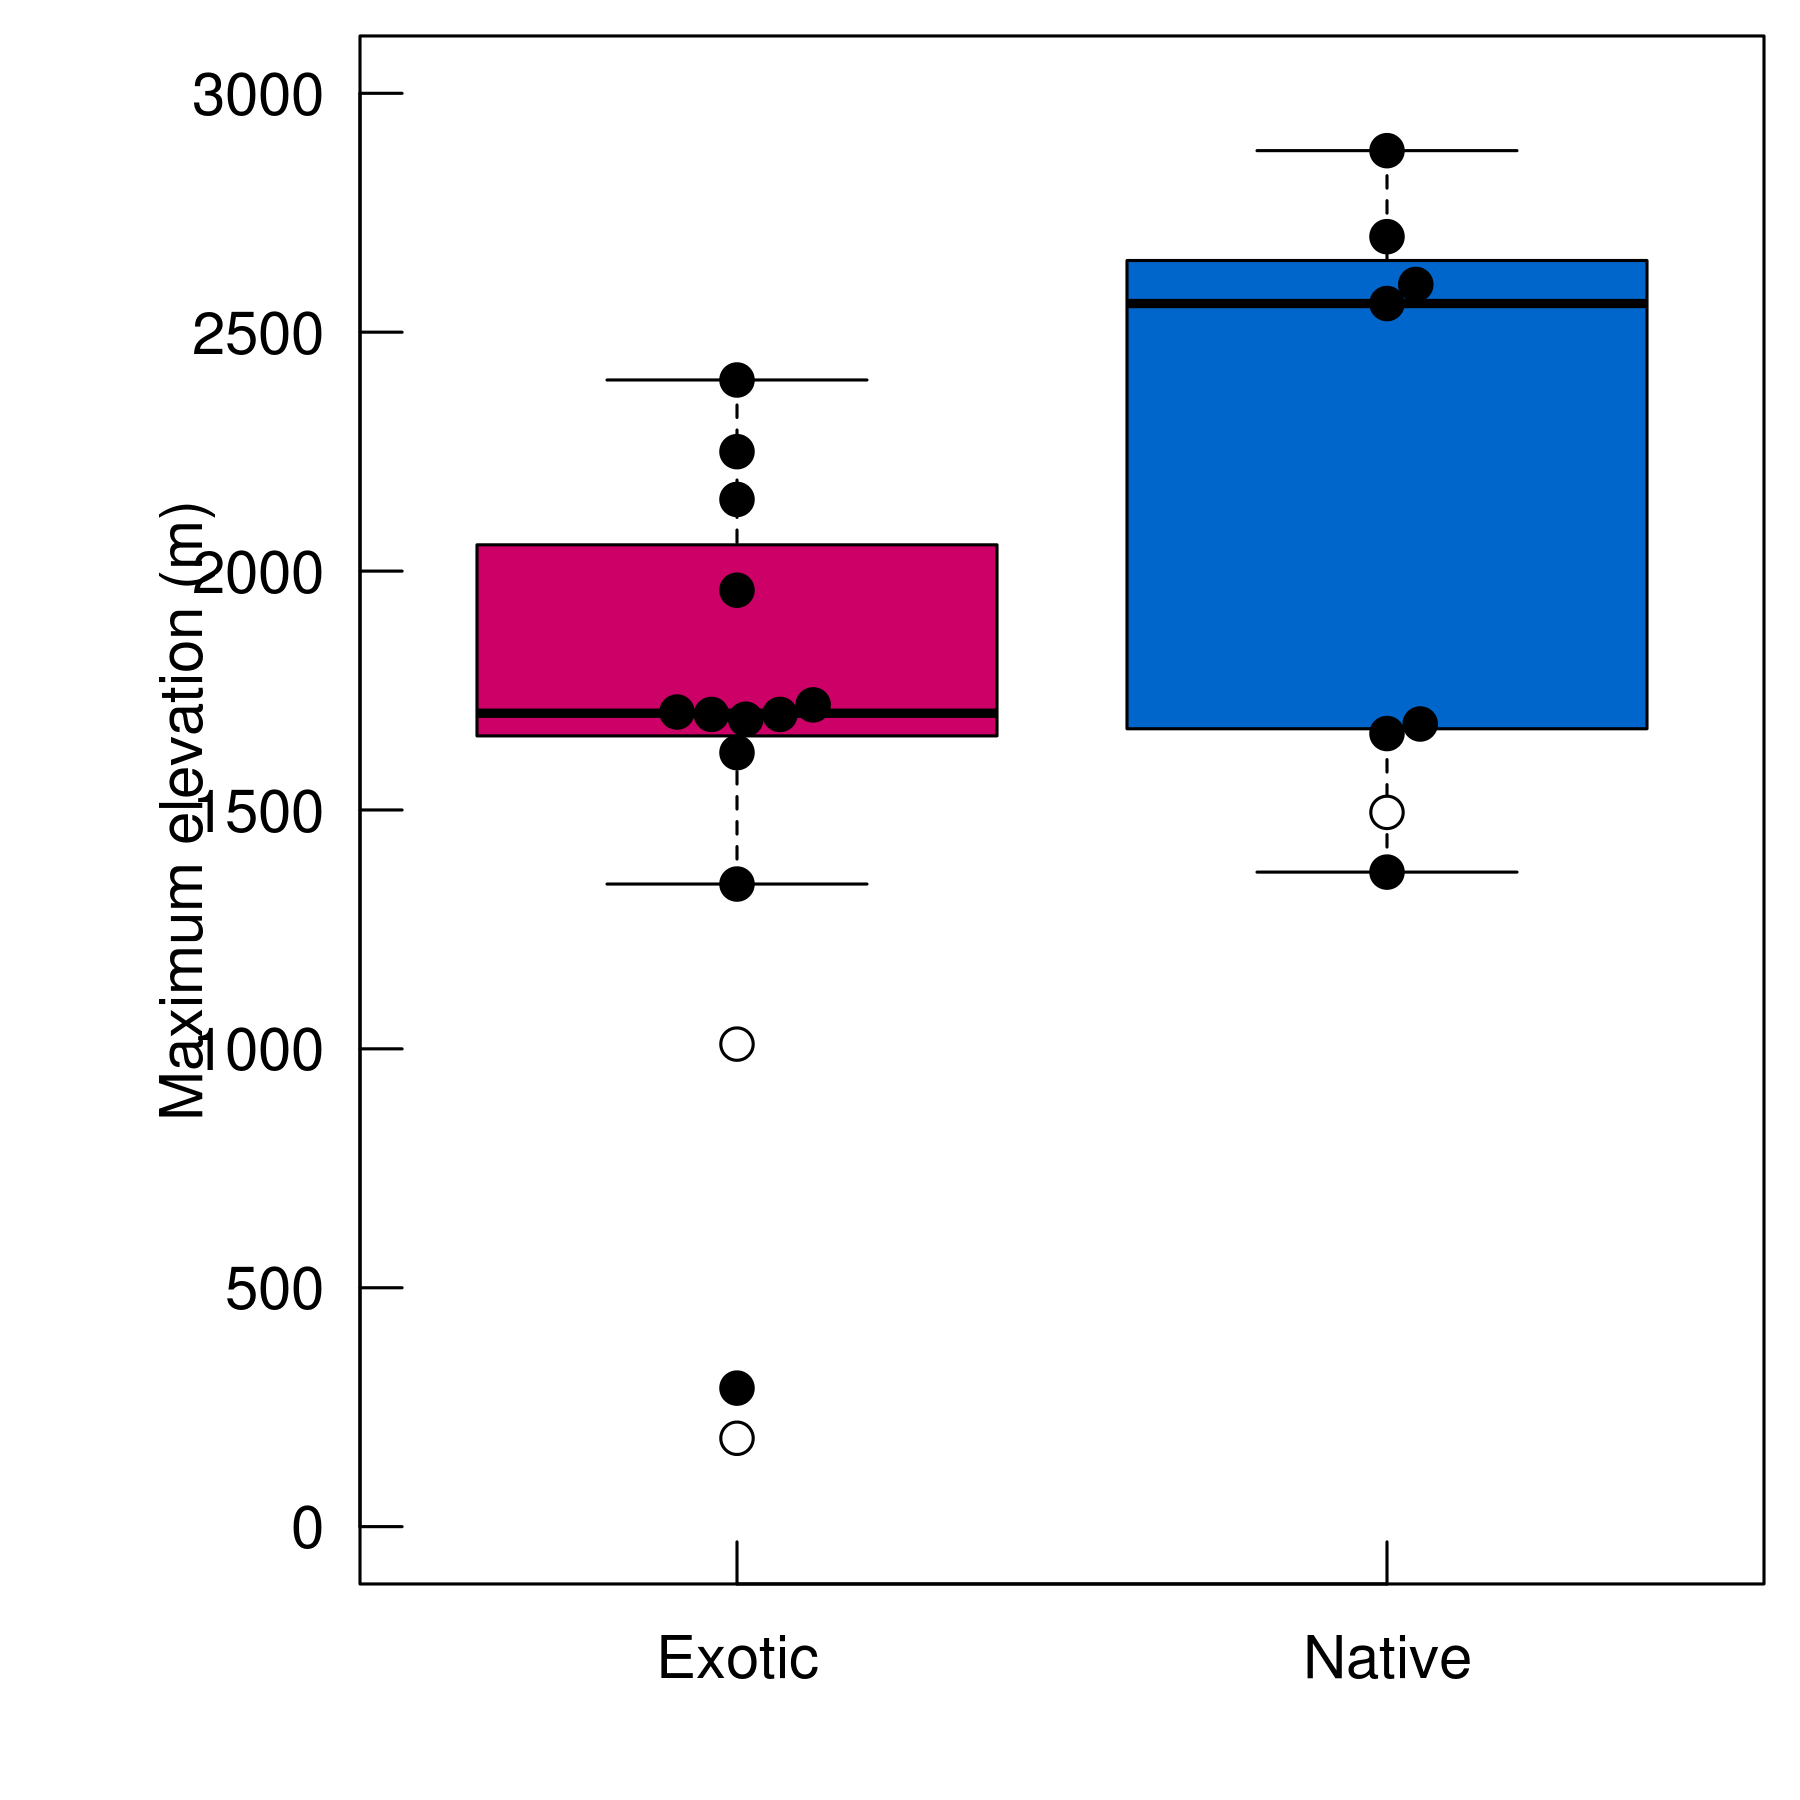
\includegraphics[width=0.7\textwidth]{figures/zoizos-boxmax}
\end{tabular}
\caption{\label{boxrange}}
\end{figure}

% % % % % % % % % % % % % % % % % % % % % % % % % % % % % % %
% % GAM FITS
\clearpage


\begin{figure}
\hspace{-2cm}
\begin{tabular}{cc}
a& b\\
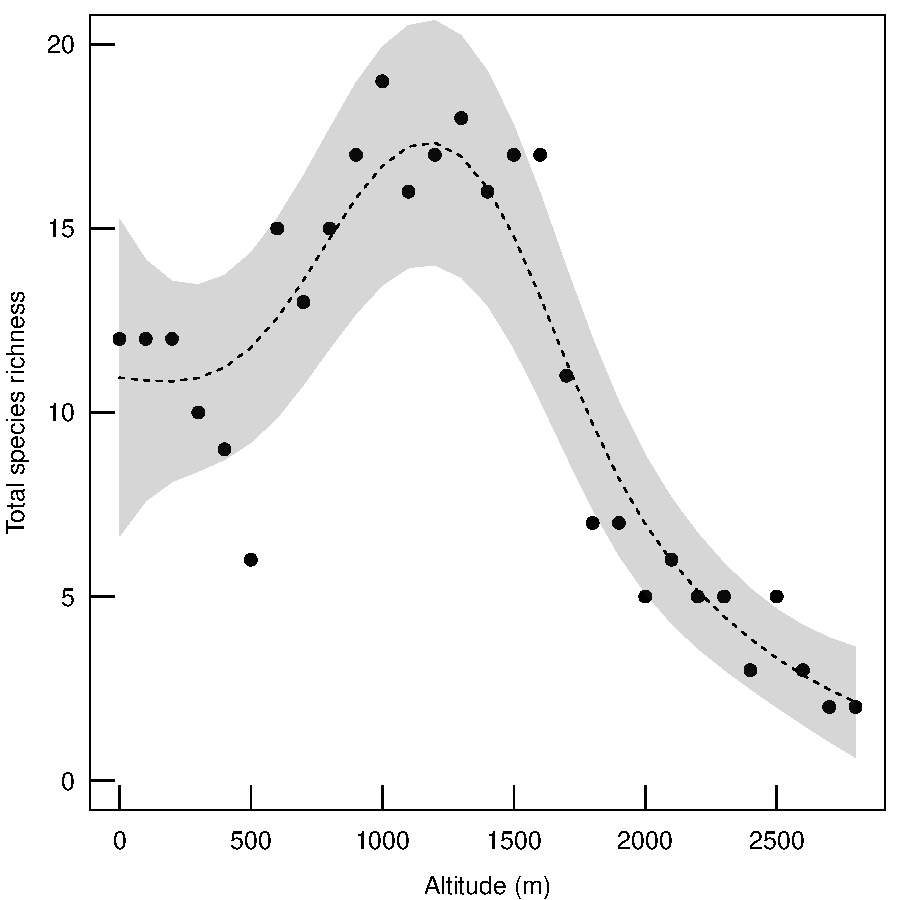
\includegraphics[width=0.7\textwidth]{figures/zoizos-Stot}
&
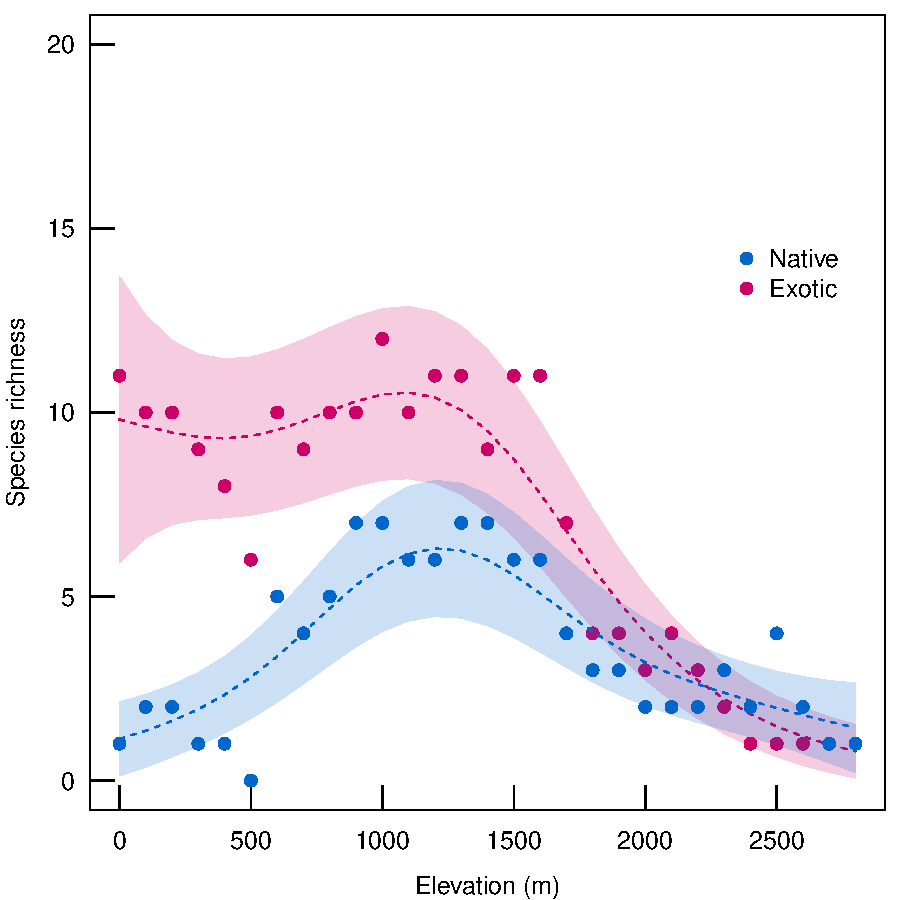
\includegraphics[width=0.7\textwidth]{figures/zoizos-Snatexo}
\end{tabular}
\caption{\label{Sgam}}
\end{figure}

\clearpage

% % NULL MODEL BOTH MARGINS

% % NULL MODEL COLUMN MARGIN PRESERVED

\begin{figure}
\hspace{-2cm}
\begin{tabular}{cc}
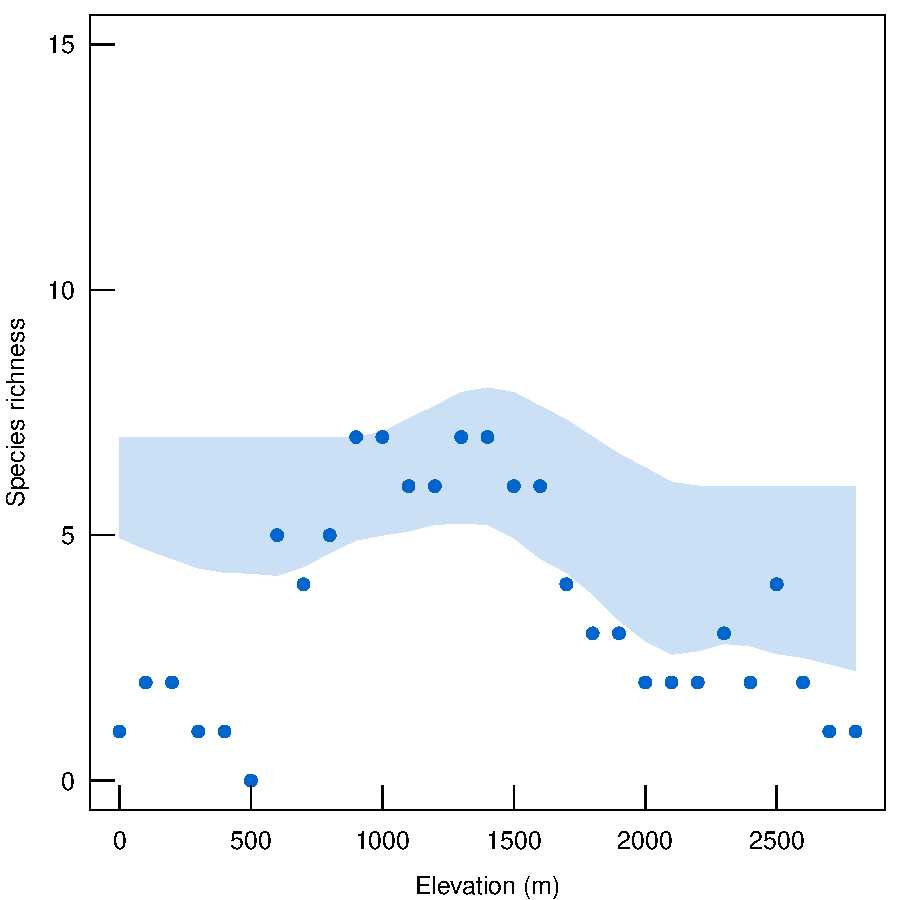
\includegraphics[width=0.7\textwidth]{figures/zoizos-Snatc}
&
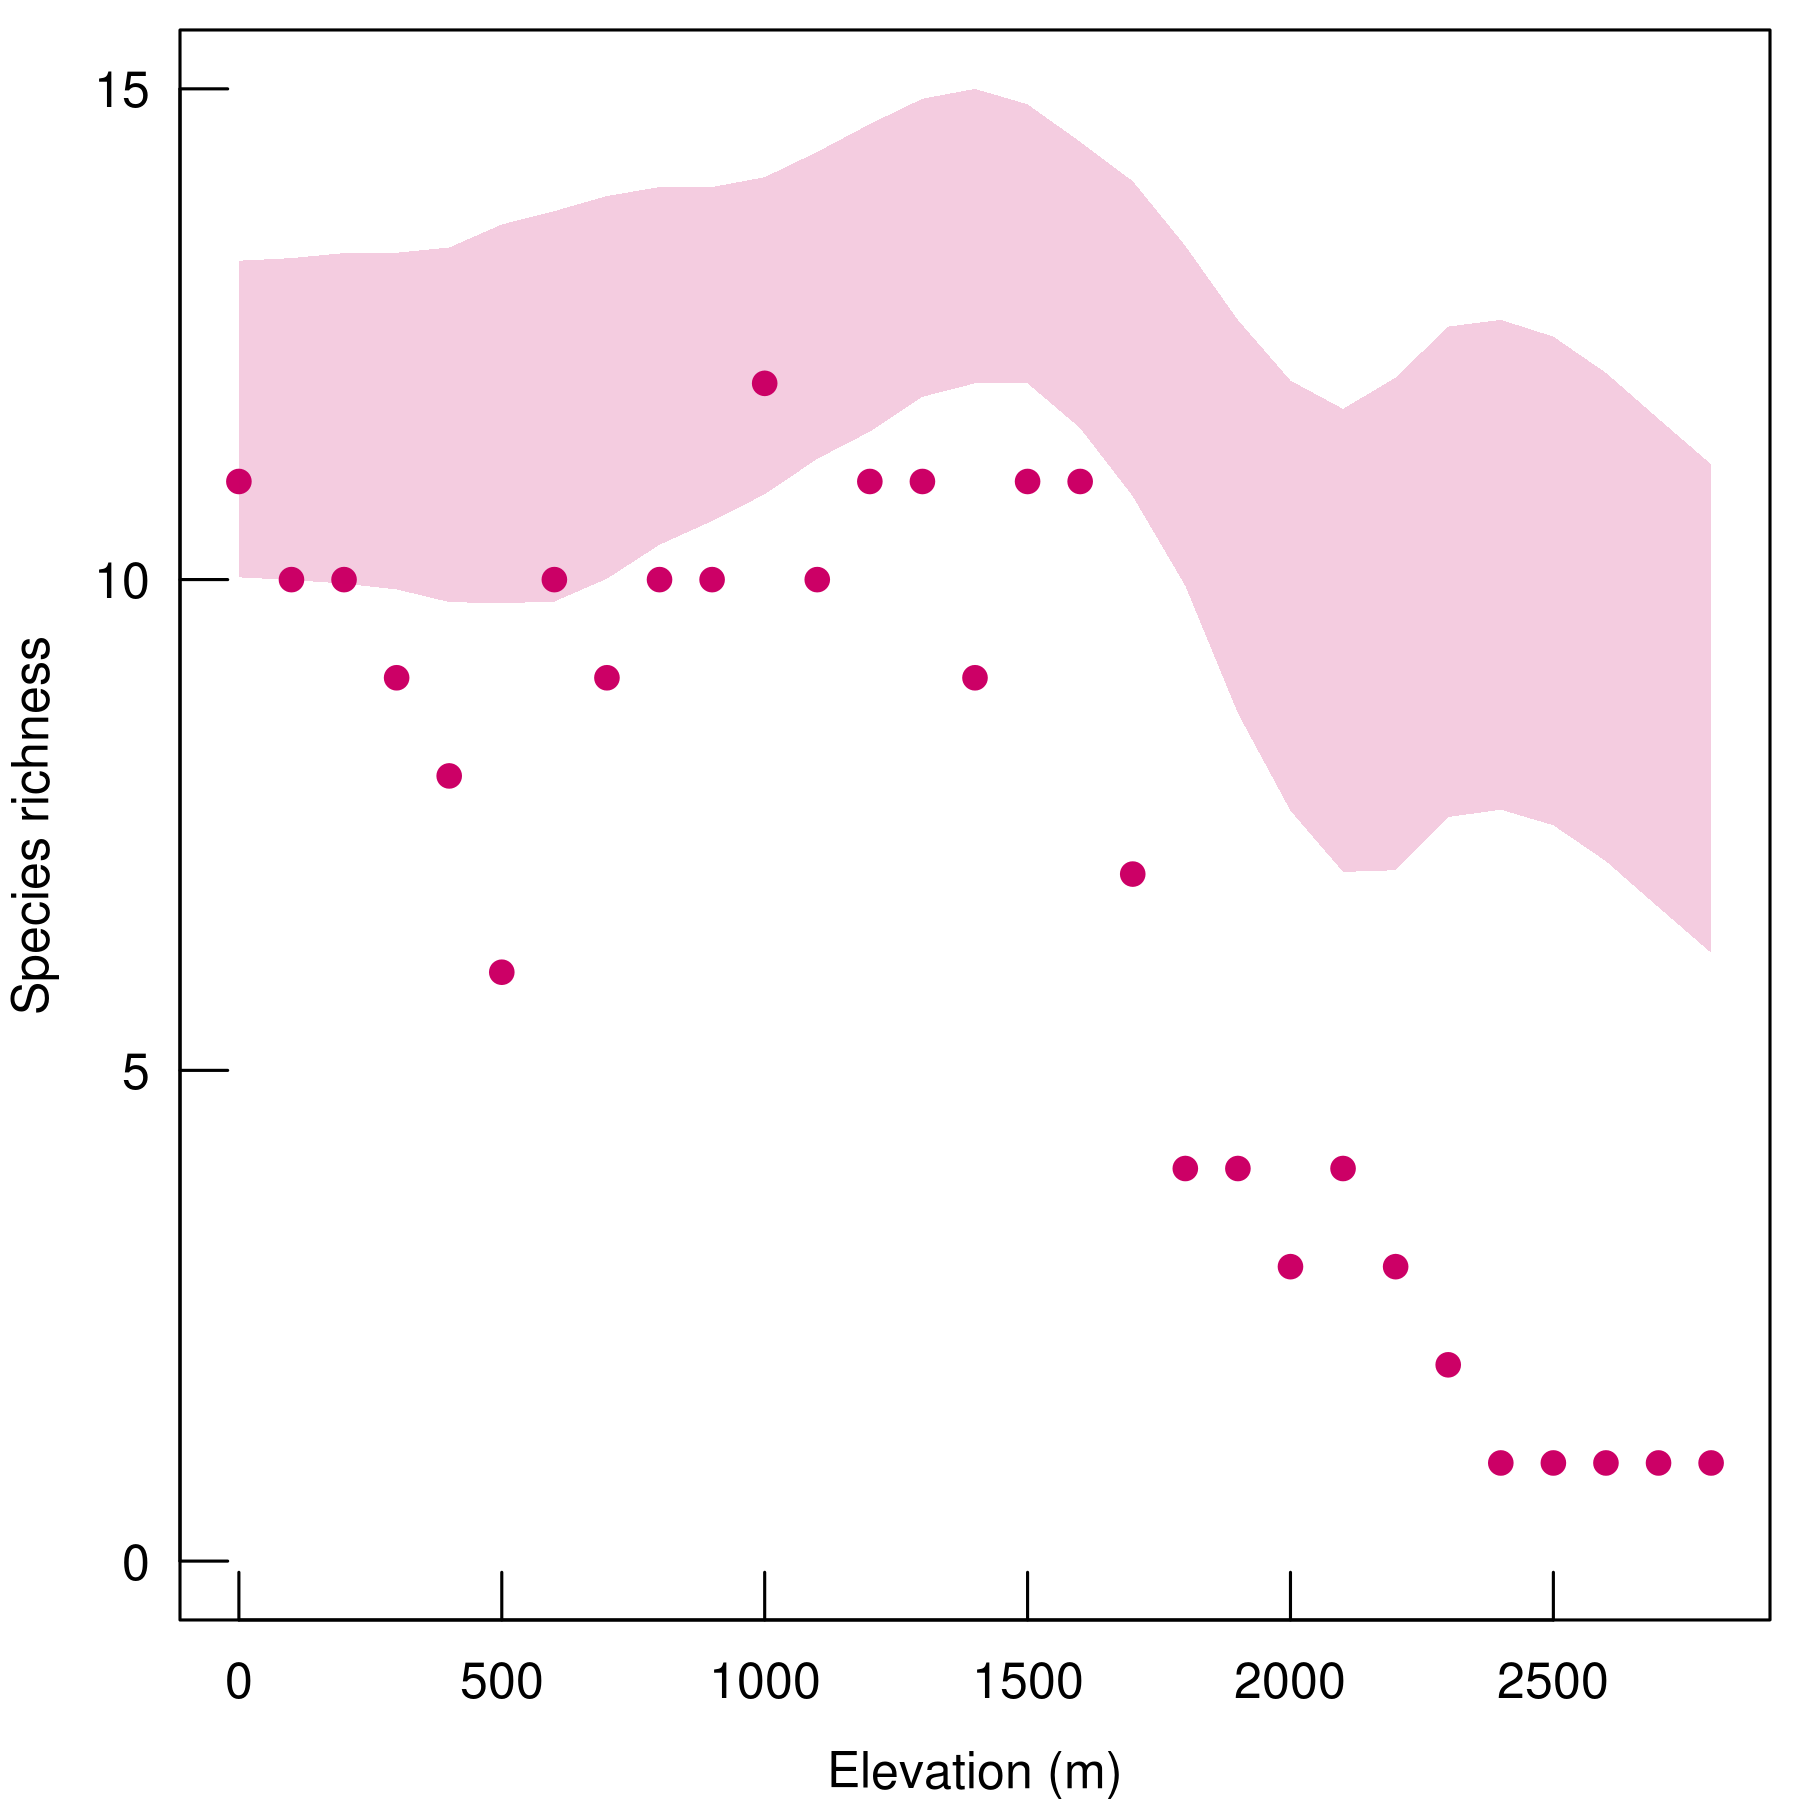
\includegraphics[width=0.7\textwidth]{figures/zoizos-Sexoc}\\

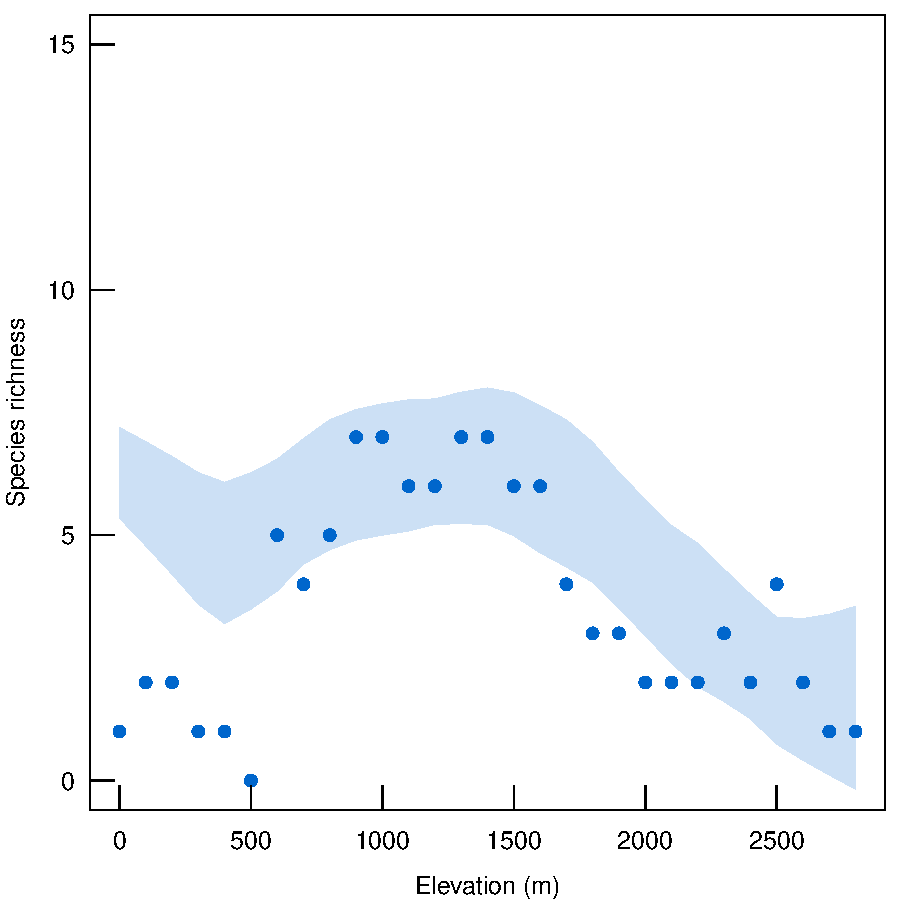
\includegraphics[width=0.7\textwidth]{figures/zoizos-Snatb}
&
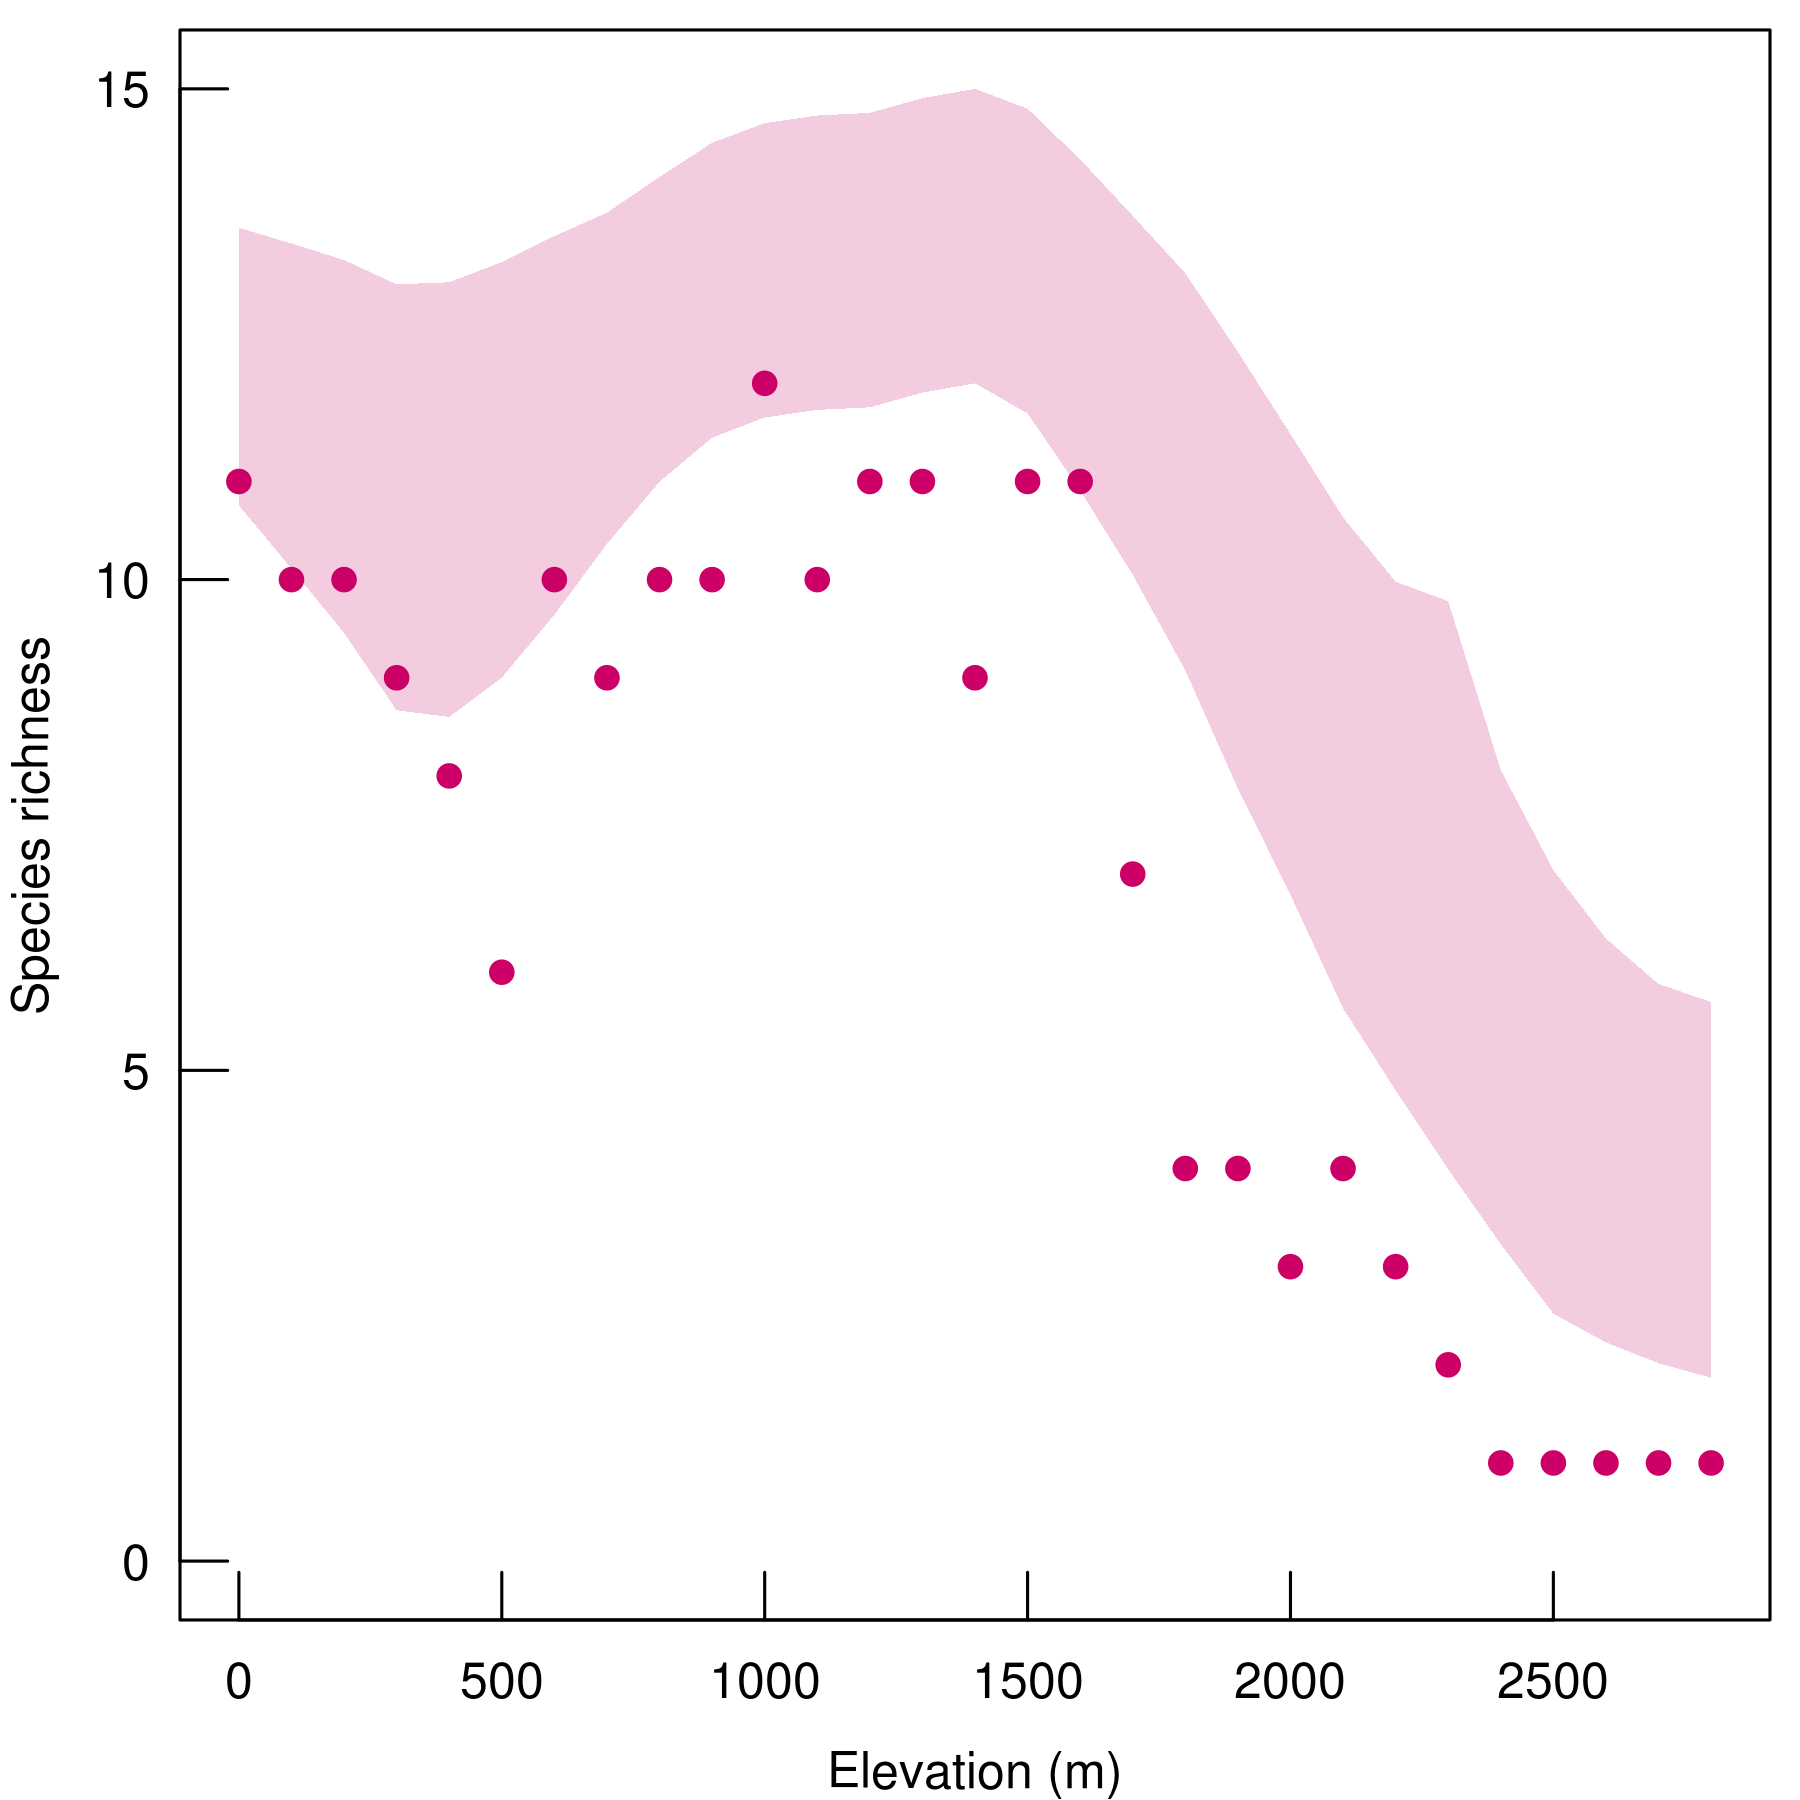
\includegraphics[width=0.7\textwidth]{figures/zoizos-Sexob}
\end{tabular}
\caption{\label{Snull}}
\end{figure}

% % % % % % % % % % % % % % % % % % % % % % % % % %
\clearpage
\section*{Supporting information}
\renewcommand{\thefigure}{S\arabic{figure}}
\setcounter{figure}{0}

\renewcommand{\thetable}{S\arabic{table}}
\setcounter{table}{0}
\begin{table}
\caption{List of bird species detected in the study\label{tbl:species}}
\footnotesize
\begin{tabular}{|llllcccc|}
\toprule
\multicolumn{1}{|c}{\textbf{Label}}& \multicolumn{1}{c}{\textbf{Species}} & \multicolumn{1}{c}{\textbf{Order}} & \multicolumn{1}{c}{\textbf{Family}} & \textbf{Mass} (g) & \textbf{Size} (cm) & \textbf{Status} & \textbf{RLI} \\
\midrule
ACTR & Acridotheres tristis & Passeriformes & Sturnidae & 82 – 134 & 23 – 29 & E & LC \\ 
CIMA & Circus maillardi & Accipitriformes & Accipitridae & 50 & 650 – 1000 & R  & EN  \\
COFR & Collocalia francica & Apodiformes & Apodidae & 7 – 13,3 &  & M & NT \\
COCH & Coturnix chinensis & Galliformes & Phasianidae & 31 – 41 & 12 – 15 & E & LC \\
COCO & Coturnix coturnix & Galliformes & Phasianidae & 16 & 70 - 135 & E & LC \\ 
ESAS & Estrilda astrild & Passeriformes & Estrildidae & 7 – 8 & 10 & E & LC \\ 
FOMA & Foudia madagascariensis & Passeriformes & Ploceidae & 13 & 17 – 19 & E & LC \\ 
FRPO & Francolinus pondicerianus & Galliformes & Phasianidae & 200 - 340 & 30 - 32 & E & LC \\ 
GEST & Geopelia striata & Columbiformes & Columbidae &  & 20 & E & LC \\ 
HYBO & Hypsipetes borbonicus & Passeriformes & Pycnonotidae & 22 & 51 - 57 & R  & LC \\ 
%LOPU & Lonchura punctata & Passeriformes & Estrildidae & 11 & 12 – 15 & E & LC \\ 
MAMA & Margaroperdrix madagascariensis & Galliformes & Phasianidae &  & 24 - 26 & N & LC \\ 
PADO & Passer domesticus & Passeriformes & Passeridae & 26 - 32 & 14 - 16 & E & LC \\ 
PEAS & Perdicula asiatica & Galliformes & Phasianidae & 57 - 82 & 17 & N & LC \\ 
PHBO & Phedina borbonica & Passeriformes & Hirundinidae &  & 13,5 & E & LC \\ 
PLCU & Ploceus cucullatus & Passeriformes & Ploceidae & 17 & 32 – 45 & E & LC \\ 
PYJO & Pycnonotus jocosus & Passeriformes & Pycnonotidae & 20 & 23 – 42 & E & LC \\ 
SATE & Saxicola tectes & Passeriformes & Muscicapidae & 12,5 & 10,5 – 15 & R  & LC \\ 
STPI & Streptopelia picturata & Columbiformes & Columbidae & 28 & 145 – 255 & N & LC  \\ 
TEBO & Terpsiphone bourbonnensis bourb. & Passeriformes & Monarchidae & 15 & 10 – 12 & M (R)  & LC \\ 
TUNI & Turnix nigricollis & Turniciformes & Turnicidae &  & 13 & N & LC  \\ 
ZOBO & Zosterops borbonicus borbonicus & Passeriformes & Zosteropidae & 10 & 7 – 8 & M (R)  & LC \\ 
ZOOL & Zosterops olivaceus & Passeriformes & Zosteropidae & 10,5 & 9 – 10 & R  & LC \\ 
\bottomrule
\end{tabular}
\end{table}

\end{document}
